\documentclass[11pt]{article}
% used by \maketitle :
\title{Additive Synthesis and Genetic Algorithms} 
\author{Nathan  Griffith}
\date{February 4, 2010}
% used by \begin{code}:
\usepackage{fancyvrb}
\usepackage{graphicx}
\DefineVerbatimEnvironment{code}{Verbatim}{fontsize=\small}
\DefineVerbatimEnvironment{example}{Verbatim}{fontsize=\small}
\newcommand{\ignore}[1]{}

\begin{document}
\maketitle % automatic title!

\section{Abstract}

The purpose of this project is to explore and manipulate sound in the frequency domain. To do so, a genetic algorithm is used as a gateway to a \emph{path} or \emph{space} between two sounds. 

The goal is not to simply devise a method of rendering the target sound, as this can be done without a genetic algorithm. Instead, the goal is to allow for the exploration of the \emph{path} that is generated by the algorithm. A wide range of unexplored sounds can be found between two different sounds, and this project attempts to explore that space through the use of the random mutations and alterations provided by a genetic algorithm. 

\section{Introduction}

Sound synthesis dates as far back as 1876, though the first commercially available synthesizer was not available until almost a century later. Since then, the number of available synthesizers and synthesis techniques have dramatically grown, and the impact of sound synthesis on popular music has only increased the demand for newer and `better' audio synthesizers.

Each method of synthesis produces a range of sounds that must be explored through adjusting settings or inputs. The idea of using a genetic algorithm to explore this range of audio data is not new. Other approaches have included Michael Chinen and Naotoshi Osaka's 2007 paper on \emph{Genesynth}\cite{genesynth}, as well as Matthew Yee-King as Martin Roth's 2008 paper on \emph{Synthbot}\cite{synthbot}. However, while not new, this approach is certainly not common, and deserves much more exploration.

This project uses a combination of a genetic algorithm and a simple additive synthesis model, which uses sound data that has been split-up into individual partials or harmonics. To render audio, each partial is passed through a simple oscillator, and the resulting waves are summed together to produce the final sound. Discussed in this paper are the details of the genetic algorithm, the rendering process, and various customization options.

In order to run, this project requires Paul Hudak's Euterpea, which can be found at the following location:
\begin{code}
http://code.haskell.org/Euterpea
\end{code}

\section{The Genetic Algorithm}

The genetic algorithm used in this project follows a fairly standard format. Given a {\bf starting sound} and a {\bf target sound}, incremental, random changes are applied to the starting sound. With each generation, a population of the ``most fit'' sounds are carried onto the next iteration of the algorithm. This ``fitness'' determination can be any form of comparison to the {\bf target sound}. Once the algorithm stops, each generation is stored in a history list. The algorithm will stop running after a specified number of generations, or after the sound has converged to match the target sound. The test for convergence simply determines if the ``fitness'' is below a certain threshold.

\subsection{Mating and Mutation}

With each generation, the algorithm makes incremental changes to the population through the use of {\bf mating} and {\bf mutation}. 

The default method for mating involves crossing-over, which takes two sounds (represented by lists of partials or harmonics) and inter-mingles the partials to create a completely new sound, which consists of approximately 50\% of each original sound. This approach is very similar to \emph{chromosomal crossover} in DNA, albeit quite simplified.
The supplied methods for mutation involve altering either the amplitude or the frequency of one of the partials, given a specified range. For example, given a range of say 100.0 Hz, a mutation would alter the frequency by adding or subtracting a random number from 0-100.
\subsection{Fitness}

The default `fitness' function involves a comparison between the current sound and the {\bf target sound}. This comparison consists of a summation of the differences between partial pairs, determined through the overall difference between both frequency and amplitude/envelope data. The closer the resulting number to zero, the closer the two sounds are.

\subsection{More Detail}

For a more code-oriented explanation, pseudocode has been included to further explain the approach used by this algorithm. Notice that a fixed population size is maintained across iterations.

\begin{code}
history = empty
current_population = starting_sound
loop: repeat until converged, or until reached max_iterations
  mutated_values = apply mutations to current_population
  mated_values   = mate members of current_population with each other
  new_population = mutated_values + mated_values + current_population
  
  loop: for each member of new_population
    determine `fitness' by comparing to target_sound
  :end loop
  sort new_population by `fitness'
  
  check the best `fitness' value for convergence (below a certain threshold)
  if (converged)
    break from loop
  else
    store best value in history
  
  current_population = the 5 `best fit' values from new_population
:end loop
\end{code}
 
\section{The Exploration}

To start exploring the results of the genetic algorithm, one must simply point {\bf ghci} to the file ``SoundDataLibrary.lhs,'' which has a number of default functions and instruments. Next, one must choose a starting sound, a target sound, the maximum number of iterations the algorithm should run (before halting or converging), and the name of the output (i.e. ``out.wav''). 
From this point, two different approaches can be taken, involving two different types of sound data.

Note that sounds such as \emph{hornBasic} and \emph{guitarBasic} are already defined in ``SoundDataLibrary.lhs.'' A number of other example instrument sounds have been included in this file.

\subsection{Approach 1}

The first approach involves {\bf basic} sound data. This type has been called `basic' because it does not account for any change in amplitude or frequency. In other words, each partial consists of a static frequency and amplitude pair. The rendering function simply takes the results of the genetic algorithm (the `history') and renders it in very fast sequence, creating an unbroken audio stream. The beginning of this audio stream sounds like the starting value, and the end sounds like the target value (only if the algorithm ran enough iterations to converge, of course).

A call to this function looks like the following:

\begin{code}
> simpleBasic hornBasic guitarBasic 1000 "horn_to_guitar_basic.wav"
\end{code}

This function results in an audio file that begins on one tone and converges over time to another tone, as shown in the following image:

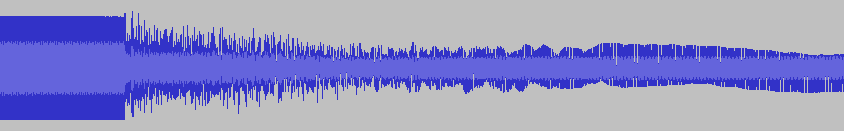
\includegraphics[width=120mm]{basic_wav.png}

\subsection{Approach 2}

The second approach involves {\bf normal} sound data. Unlike the `basic' type, the `normal' type uses an {\bf envelope} to account for changes in amplitude over time. As one might expect, when directly rendered to audio, a `normal' sound data sounds much more realistic than its `basic' cousin. When rendering the results of the genetic algorithm on `normal' data, a function can be used to play selections from the `history' one-by-one, instead of in fast sequence.

\begin{code}
> simpleNormal hornNormal guitarNormal 1000 "horn_to_guitar.wav" 30.0 
\end{code}

Note that \emph{simpleNormal} also takes a duration value (in this case, 30.0 seconds), which tells it the maximum length of audio to render.
The resulting audio file looks something like this:

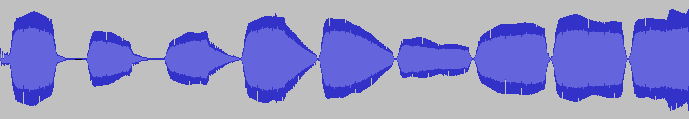
\includegraphics[width=120mm]{normal_wav.png}

\section{Further Customizing the Algorithm}

While these basic functions are supplied, a number of abstractions exist which allow for the detailed customization of portions of the algorithm. This can be accomplished by including the relevant project files in the header of a custom haskell module:

\begin{code}
> module MyCustomizations where
> import SoundData
> import SoundDataMutate --I plan to write some custom mutation functions
> import SoundDataGeneRun --I will then require a call to the GA
\end{code}

After this is done, direct calls can be made to the GA using the following commands:

\begin{code}
> runBasic  x mut_ops mut_prob fitness_fn start target
> runNormal x mut_ops mut_prob fitness_fn start target
\end{code}

Where \emph{x} is the maximum number of iterations, \emph{mut-ops} is a list of mutation functions, \emph{mut-prob} is the probability, out of 100, that a mutation will occur, \emph{fitness-fn} is the fitness or comparison function, and the \emph{start} and \emph{target} values are `basic' or `normal' sound data types (depending on the type of the function being used). An actual call to such a function might look as follows:

\begin{code}
> runBasic 1000 [mutateFreqB gen,mutateAmplB gen,big_mutateFreqB gen]
>            100 crossoverBasicPop hornBasic guitarBasic
\end{code}

This will generate an array of sound data values of length 1000 (one for each generation). Because it is simply a list, the haskell operator (!!) may be used to extract any individual sound data. An individual sound data may then be rendered with one of the following functions:

\begin{code}
> renderSoundB name dur data
> renderSoundN name dur data
\end{code}

Where `name' is the name of the audio file (``out.wav''), `dur' is the duration of the audio to be rendered (in seconds), and data is a sound data value.

\subsection{Instruments}

A number of built-in instruments have been supplied. The \emph{basic} types include `hornBasic,' `guitarBasic,' `stringsBasic,' `organBasic,' `pianoBasic,' `voiceBasic,' and `otherBasic.' Similarly, the \emph{normal} types include `hornNormal,' `guitarNormal,' `stringsNormal,' `organNormal,' `pianoNormal,' `voiceNormal,' and `otherNormal.' 
To hear what each of these sounds like, one could manually render the sound data using one of the previous commands, or use a built-in test-render that has been supplied for each instrument:

\begin{code}
> hornListen
> guitarListen
...
> voiceListen
\end{code}

Each of these intruments can be found in ``SoundDataLibrary.lhs.'' Custom instruments can be added following the same data format as the built-in instruments. Note that data from the built-in instruments was extracted from the program SPEAR by Michael Klingbeil\cite{klingbeil}, though any software which lists partial/harmonic data line-by-line could be used and formatted for input.

\subsection{Mutations}

The \emph{runBasic} (or \emph{runNormal}) function takes a list of mutation functions as the \emph{mutOptions} argument. One such list, with mutation functions for manipulating both the frequency and amplitude of a \emph{SoundPartial}, might look as follows:

\begin{code}
> mutOptionsB :: (RandomGen g) => g -> [SoundRoot -> (SoundRoot,g)]
> mutOptionsB gen = [mutateFreqB gen,mutateAmplB gen]
\end{code}

This allows for the specification and customization of any number of mutation functions. If, for instance, one were not satisfied with the number of generations required for partials to change frequency, a completely new mutation function could be specified which would allow individual partials to leap long distances (up to 500Hz in this case) with each generation\footnote{While this approach would cause \emph{SoundData} types with large differences in frequency to converge more rapidly early on, this function would only become a nuisance when the algorithm attempts to fine-tune the frequency of each partial. One should attempt to strike a balance between the initial speed of convergence, which should be fast, and the ability for mutations to make very small adjustments during later iterations.}:

\begin{code}
> -- mutate the frequency of a SoundRoot (very large leaps)
> mutateFreqB_BIG :: (RandomGen g) => g -> SoundRoot -> (SoundRoot,g)
> mutateFreqB_BIG gen (Sine f a) = ((Sine new_f a),new_gen)
>   where out = (mutateDouble gen 500.0 f)
>         new_gen = snd out
>         new_f = fst out
\end{code}

Note that each mutation function, as well as the list of mutation functions, takes a random number generator as an argument. In addition, the mutation functions return both the modified partial and a new generator for later use. Because the generator is explicitly passed to the function, one can generate as many random numbers as needed, including none at all. In other words, the exact purpose of the \emph{randomness} can be hand-tailored for each function.

\subsection{Mating and Crossover}

Similar to the mutation function, the mating function can also be customized and passed to one of the GA iterators. If, for instance, one were not satisfied with the way the default crossover function is applied to all possible pairings within a population, one could write something like the following, which zips the population list with its reverse, forming fewer pairings:

\begin{code}
> --crossover a list of BASIC sound datas
> myCrossover :: (RandomGen g) => [BasicSoundData] -> g -> [BasicSoundData]
> myCrossover lst gen = zipWith crossoverBasic lst (reverse lst)
\end{code}

\subsection{The Fitness Function}

As one might expect, the fitness function itself can be customized. The default takes both amplitude and frequency into account. One could write a much simpler function that ignores amplitude entirely. If coupled with a lack of amplitude mutation functions, this could result in an output that consists of entirely new frequencies (as usual) but amplitude data that is identical to that of the starting value. This function might look like the following:

\begin{code}
> compareBasic :: BasicSoundData -> BasicSoundData -> Double
> compareBasic a b = (helper (zip (sortBasic a) (sortBasic b))) + (fromIntegral diff)
>   where
>     helper sbPairs = foldr (+) 0 (map (\(a,b) -> (compareRoot a b)) sbPairs)
>     compareRoot (Sine a _) (Sine c _) = abs (a - c) --NO AMPLITUDE COMPARISON
>     diff = abs ((length a) - (length b)) --difference in length
\end{code}

\subsection{Rendering}

Finally, while functions are provided to render the results of the genetic algorithm in certain ways, one could write any number of functions to manipulate the sound data before it is rendered. This could include modulations in frequency, normalization of amplitude, or perhaps linear morphing between `basic' types. There is no limit, as the render functions (\emph{renderSoundB}, \emph{renderSoundN}, and \emph{renderSoundC}) are designed to work with anything that fits within the confines of the {\bf SoundData} type, specified in ``SoundData.lhs.''

\section{Conclusion}

The \emph{space} that exists between two sounds is quite vast, containing almost limitless variations, and in many cases remains largely unexplored. This algorithm attempts to reveal much of this unexplored territory, and might be a tool for modern composers and producers to find new and unique sounds. 

In summary, this project can be used to easily create sounds using any of the built-in defaults, or can be tailored for any specific need. While plenty of default options have been provided, the real utility lies in customizing the algorithm and using the \emph{SoundData} type for one's own purposes. 

\begin{thebibliography}{2}

	\bibitem{genesynth}
	  Michael Chinen and Naotoshi Osaka,
	  \emph{Noise Band-based Genetic Algorithm Analysis/Synthesis Framework}.
	  Tokyo Denki University,
	  2007.
	\bibitem{synthbot}
	  Matthew Yee-King, Martin Roth,
	  \emph{Synthbot: An Unsupervised Software Synthesizer Programmer}.
	  International Computer Music Conference,
	  2008.
	\bibitem{klingbeil}
	  Michael Klingbeil,
	  \emph{SPEAR}.
	  www.klingbeil.com/spear.
\end{thebibliography}
\end{document}             % End of document.
